\documentclass[a4paper,10pt]{article}
\usepackage[utf8]{inputenc}
\usepackage{graphicx}
\usepackage{amsmath}
\usepackage{amssymb}
\usepackage{hyperref}
\usepackage{caption}
\usepackage{subcaption}

\newcommand{\mb}[1]{\ensuremath{\mathbf{#1}}}
\newcommand{\mc}[1]{\ensuremath{\mathcal{#1}}}
\newcommand{\mbb}[1]{\ensuremath{\mathbb{#1}}}

%opening
\title{Solution of the fourth exercise assignment}
\author{Lucas Nogueira Ribeiro - 373082}
\date{}

\begin{document}

\maketitle

\section{Introduction}
Linear methods such as Least-squares estimators, Fisher's Linear Discriminant, Multiclass Logistic Regression, were employed to solve classification problems in this exercise assignment.

\section{Methodology}
Python scripts were written to solve this assignment. The sourcecode is available in the Jupyter notebook format at 
 \url{https://github.com/lnribeiro/patternrecognition/blob/master/4th%20assignment/4th_assigment.ipynb}.

\section{Results}

\subsection*{First exercise}
The obtained mean square error (MSE) and sum-of-square error are
\begin{verbatim}
 MSE [train]: 0.0190868610825
 MSE [test]: 0.0188001558568
 Sum-of-squares error [test]: 9.40007792838
 Sum-of-squares error [train]: 28.6302916237
\end{verbatim}
Data from the test set and the decision boundary are plotted in Figure \ref{fig:1f1}. The obtained classification rate is 100\%.
\begin{figure}[htb]
 \centering
 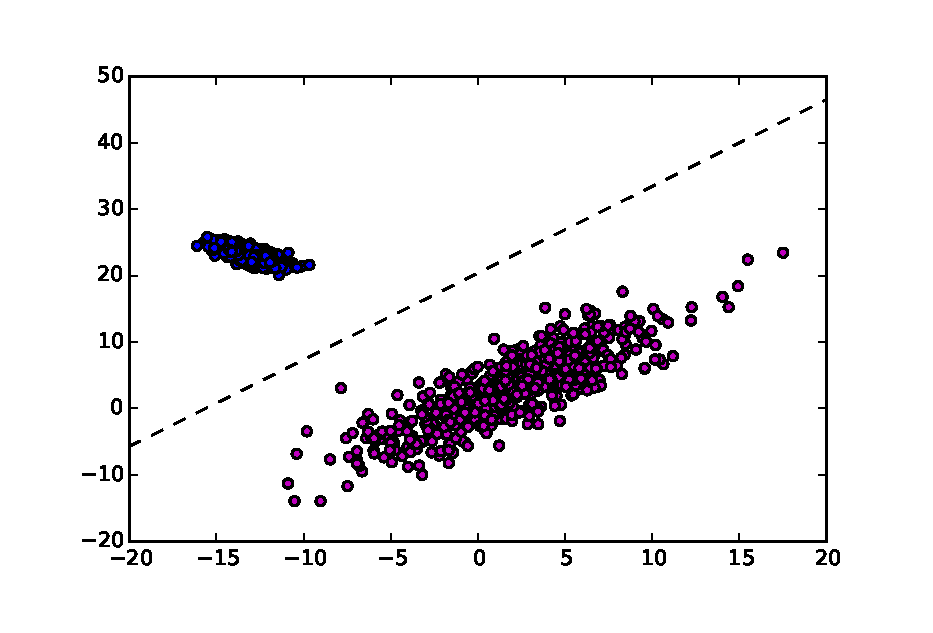
\includegraphics[scale=0.7]{./figures/1f3.eps}
 \caption{Test dataset and its decision boundary}
 \label{fig:1f1}
\end{figure}

\cleardoublepage
\subsection*{Second exercise}
The generated dataset and its decision boundary, obtained using Fisher's Linear Discriminant, are plotted in Figure \ref{fig:2f1}. The obtained classification rate was 100\%.
\begin{figure}[htb]
 \centering
 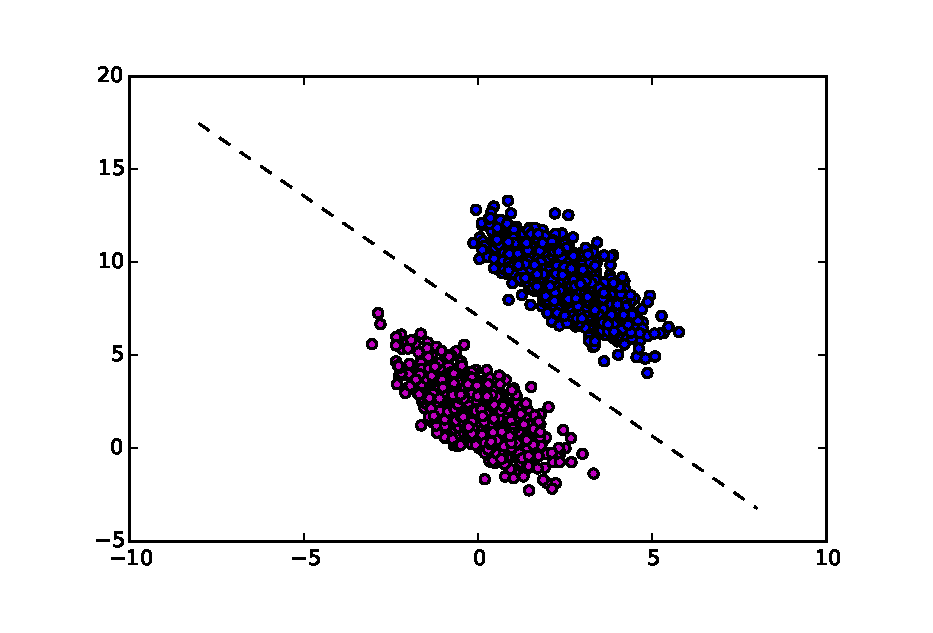
\includegraphics[scale=0.7]{./figures/2f2.eps}
 \caption{Generated dataset and its decision boundary, which was calculated using the Fisher's Linear Discriminant.}
 \label{fig:2f1}
\end{figure}

\cleardoublepage
\subsection*{Third exercise}
The decision boundaries obtained using a Perceptron in the data of the 1st and 2nd questions are depicted in Figures \ref{fig:3f1} and \ref{fig:3f2}, respectively. Although the boundaries seem to be misplaced, the obtained classification rates for both data are 100\%. The Perceptron algorithm is indeed capable of providing high classification rates given that the data is linearly separable. In practical scenarios, however, data seldom satisfies this condition. Multilayer perceptron classifiers are more adapted to real scenarios.
\begin{figure}[htb]
 \centering
 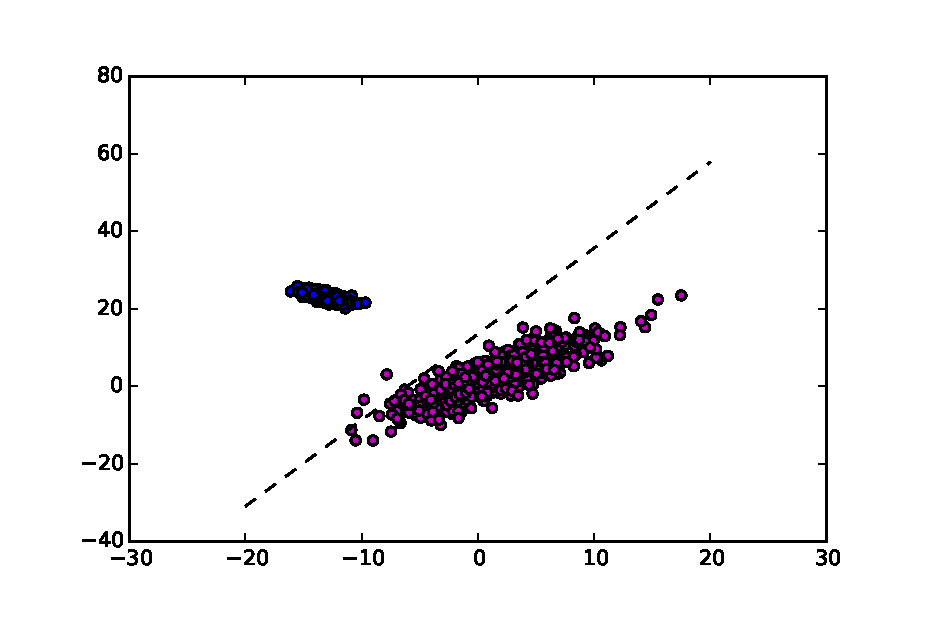
\includegraphics[scale=0.6]{./figures/3f1.eps}
 \caption{Generated dataset and its decision boundary, which was calculated using the Fisher's Linear Discriminant.}
 \label{fig:3f1}
\end{figure}
\begin{figure}[htb]
 \centering
 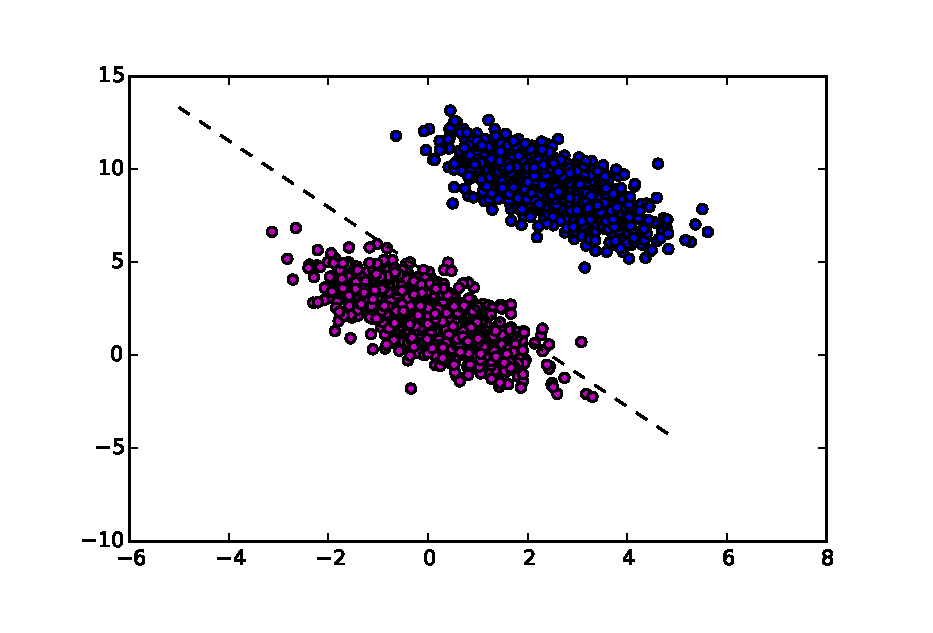
\includegraphics[scale=0.6]{./figures/3f2.eps}
 \caption{Generated dataset and its decision boundary, which was calculated using the Fisher's Linear Discriminant.}
 \label{fig:3f2}
\end{figure}

\cleardoublepage
\subsection*{Fourth exercise}
The train dataset is illustrated in Figure \ref{fig:4f1}. The decision boundaries for the red, blue, and green classes are depicted in Figures \ref{fig:4f2}, \ref{fig:4f3}, and \ref{fig:4f4}, respectively. These boundaries are plot together in Fig.~\ref{fig:4f5}. The classification rate in the test dataset was 99.83\%.
\begin{figure}[htb]
 \centering
 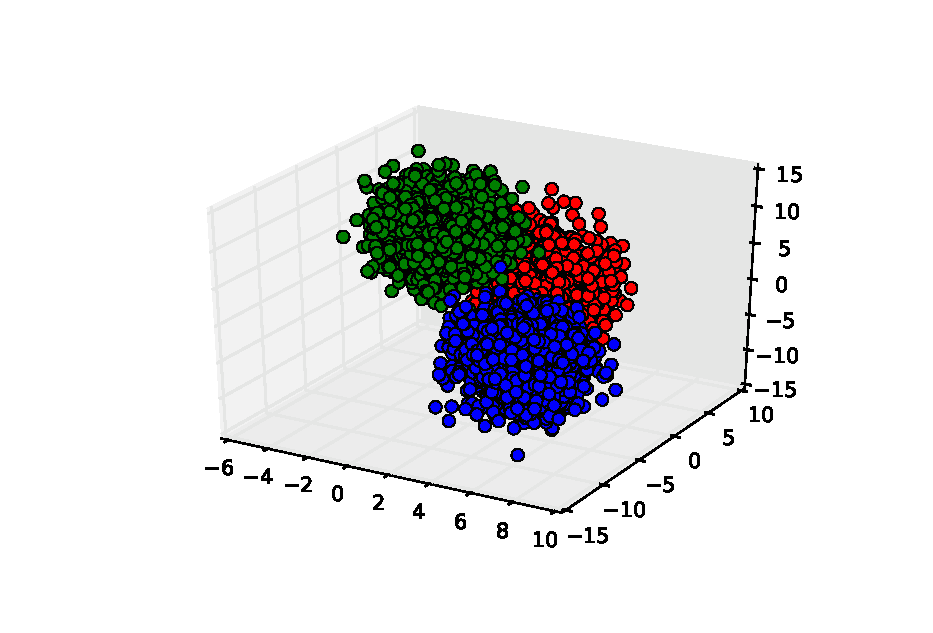
\includegraphics[scale=0.6]{./figures/4f1.eps}
 \caption{Train dataset}
 \label{fig:4f1}
\end{figure}

\begin{figure}[htb]
 \centering
 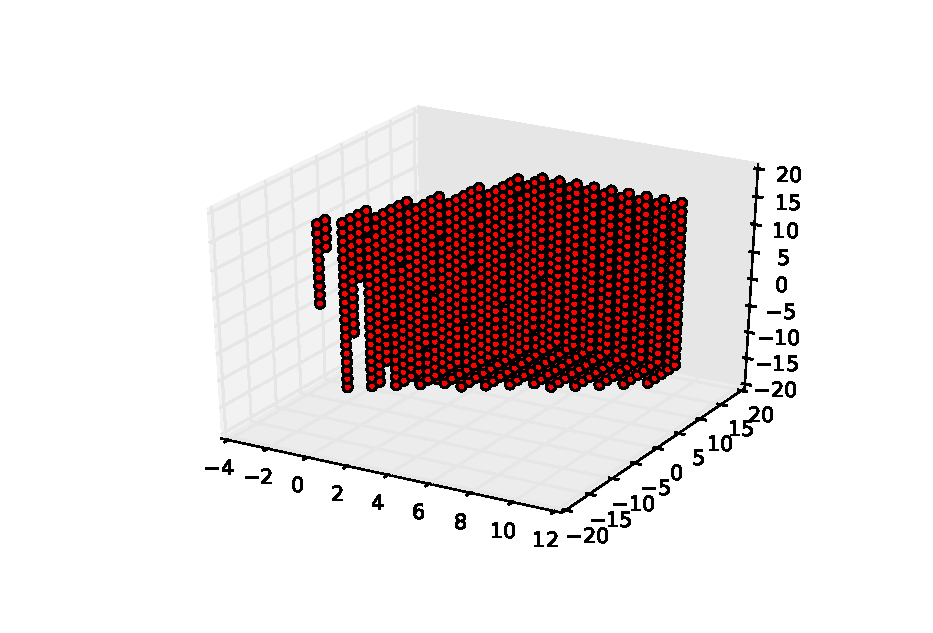
\includegraphics[scale=0.6]{./figures/4f2.eps}
 \caption{Decision boundary - red class}
 \label{fig:4f2}
\end{figure}

\begin{figure}[htb]
 \centering
 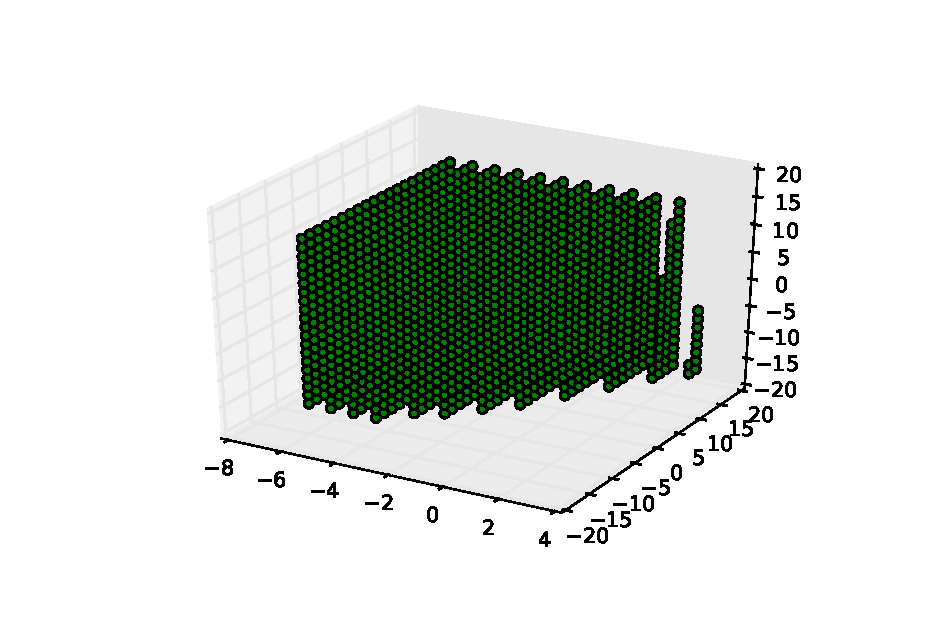
\includegraphics[scale=0.6]{./figures/4f3.eps}
 \caption{Decision boundary - green class}
 \label{fig:4f3}
\end{figure}

\begin{figure}[htb]
 \centering
 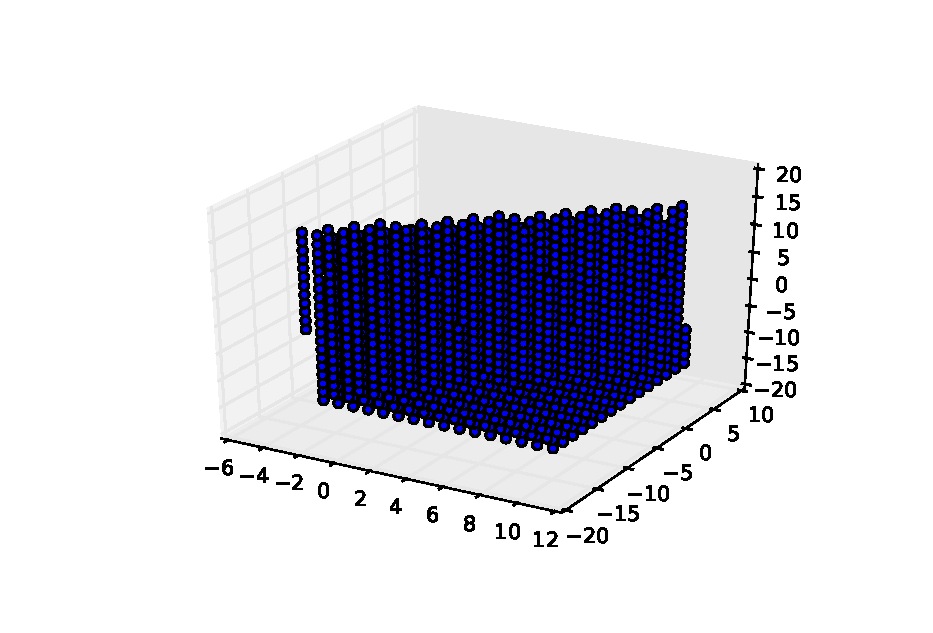
\includegraphics[scale=0.6]{./figures/4f4.eps}
 \caption{Decision boundary - blue class}
 \label{fig:4f4}
\end{figure}

\begin{figure}[htb]
 \centering
 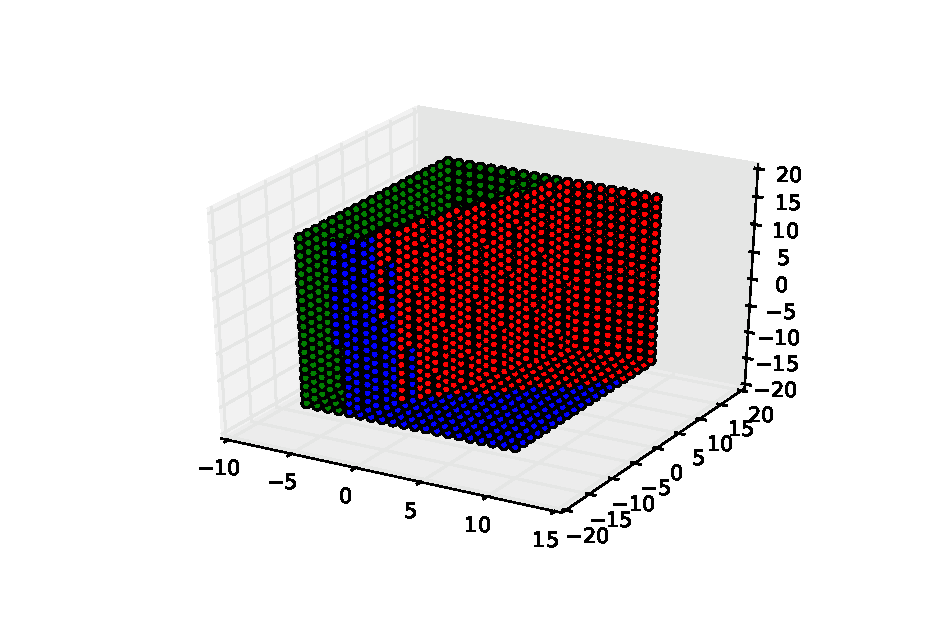
\includegraphics[scale=0.7]{./figures/4f5.eps}
 \caption{Decision boundaries}
 \label{fig:4f5}
\end{figure}

\cleardoublepage
\subsection*{Fifth exercise}
The classification rate provided by the multiclass logistic regression classifier in the test stage was 98.83\%. This rate is inferior than that provided by the probabilistic generative model in the previous exercise.

\cleardoublepage
\subsection*{Sixth exercise}
The calculated statistics of the data attributes are shown below:
\begin{verbatim}
Attribute 0: max 7.9 min 4.3 mean 5.844 +- 0.824659929911
Attribute 1: max 4.4 min 2.0 mean 3.05733333333 +- 0.434410967735
Attribute 2: max 6.9 min 1.0 mean 3.76666666667 +- 1.76218298962
Attribute 3: max 2.5 min 0.1 mean 1.19933333333 +- 0.759692627902
\end{verbatim}
PCA was employed to reduce the dimensionality of the IRIS dataset. After preserving only the two principal components of the original data, a dataset with two features was obtained. A linear classifier was used to obtain the decision boundaries. In Figure \ref{fig:6f1}, the bidimensional dataset and its decision boundaries are depicted. The average classification rate was 92.67\%.

\begin{figure}[htb]
 \centering
 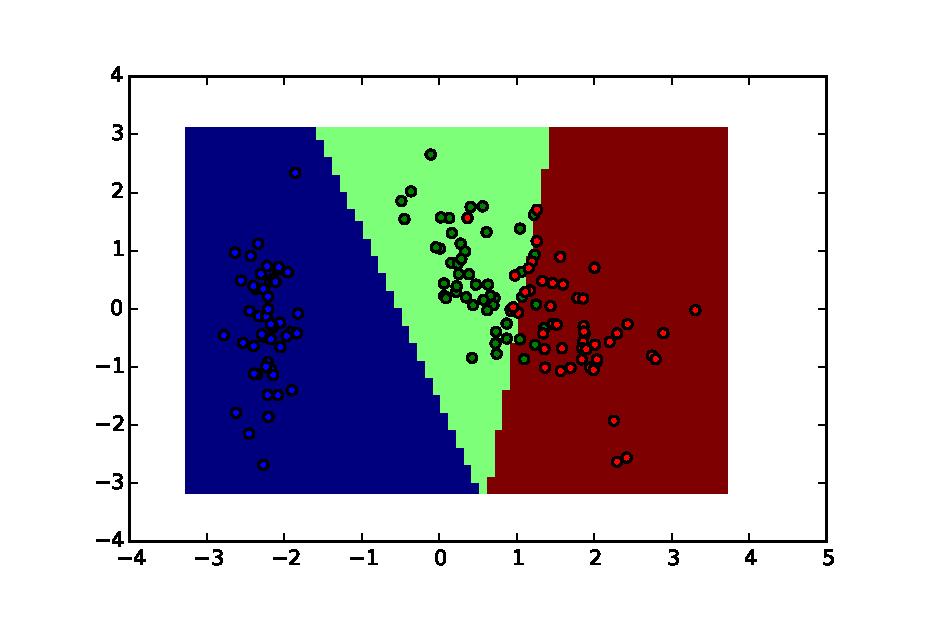
\includegraphics[scale=0.7]{./figures/6f1.eps}
 \caption{Decision boundaries considering the two principal components of the IRIS dataset.}
 \label{fig:6f1}
\end{figure}

\cleardoublepage
\section{Conclusion}
Least-squares estimators, Fisher's Linear Discriminant, Multiclass Logistic Regression and other linear methods were employed to solve the exercises proposed in this assigment. Since most of the datasets were linearly separable, good classification rates were obtained.

\end{document}
